\documentclass[twoside,twocolumn]{article}

\usepackage{blindtext} 
\usepackage{graphicx}
\usepackage[sc]{mathpazo} 
\usepackage[T1]{fontenc} 
\linespread{1.05} 
\usepackage{microtype} 


\usepackage[english]{babel} 


\usepackage[hmarginratio=1:1,top=32mm,columnsep=20pt]{geometry} 
\usepackage[hang, small,labelfont=bf,up,textfont=it,up]{caption} 
\usepackage{booktabs} 


\usepackage{lettrine} 


\usepackage{enumitem} 
\setlist[itemize]{noitemsep} 


\usepackage{abstract} 
\renewcommand{\abstractnamefont}{\normalfont\bfseries} 
\renewcommand{\abstracttextfont}{\normalfont\small\itshape} 


\usepackage{titlesec} 
\renewcommand\thesection{\Roman{section}} % 
\renewcommand\thesubsection{\roman{subsection}} 
\titleformat{\section}[block]{\large\scshape\centering}{\thesection.}{1em}{} 
\titleformat{\subsection}[block]{\large}{\thesubsection.}{1em}{} 


\usepackage{fancyhdr} 
\pagestyle{fancy} 
\fancyhead{} 
\fancyfoot{} 
\fancyhead[C]{Comparativa de herramientas de Data StoryTelling $\bullet$ Abril 2021 $\bullet$ } 
\fancyfoot[RO,LE]{\thepage} 


\usepackage{titling} 


\usepackage{hyperref} 


%----------------------------------------------------------------------------------------
%	TILULOS
%----------------------------------------------------------------------------------------


\setlength{\droptitle}{-4\baselineskip} 

\pretitle{\begin{center}\Huge\bfseries} 
\posttitle{\end{center}} 
\title{Comparativa de herramientas de Data StoryTelling} 
\author{Luis Cancino,Angel Crispin,Derian Herrera,Julio Mejia,Randy Paredeses }
\date{\today} 
\renewcommand{\maketitlehookd}{
\begin{abstract}
\noindent 
Data Storytelling is important for Narrative
 in Data Visualization is one of the
 main Big Data tools that
 business cannot be lost. Therefore, in this
 post we tell you the most interesting of Data
 Storytelling, what it is and how to improve results
  thanks to that.
In case you did not know, each time they will be needed
more big data professionals and storytellers in the
sector. The change in the digital age demands profiles
with analytical and intelligence capabilities
business. As a consequence, the new
 generations will go beyond these disciplines,
  with new ideas and spaces for business.
\end{abstract}
\begin{abstract}
\noindent 

El Data Storytelling es importante para la Narrativa
 en la Visualización de Datos es una de las
 principales herramientas del Big Data que los 
 negocios no se pueden perder. Por eso, en este 
 post te contamos lo más interesante del Data 
 Storytelling, qué es y cómo mejorar los resultados
  gracias a ello.
Por si no lo sabías, cada vez se van a necesitar 
más profesionales big data y  storytelleres en el 
sector. El cambio en la era digital demanda perfiles 
con capacidades analíticas y de inteligencia 
empresarial. Como consecuencia, las nuevas
 generaciones irán más allá de estas disciplinas,
  con nuevas ideas y espacios para los negocios.

\end{abstract}
}

%----------------------------------------------------------------------------------------

\begin{document}

% Print the title
\maketitle

%----------------------------------------------------------------------------------------
%	INTRODUCCION
%----------------------------------------------------------------------------------------

\section{Introduccion}
\lettrine[nindent=0em,lines=3]{A}
Los seres humanos están marcados con historias y
experiencias que moldean la modo del valoración 
personal. A separar del jerga comprendemos que la
ánimo es una gama de diario o anécdotas que el 
persona narra para asomar nota en sociedades o 
grupos culturales.
Gracias a las narraciones nuestros más remotos 
ancestros preservaron el conocimiento de una 
generación a la siguiente, permitiendo la 
supervivencia de la civilización (Abrahamson, 1998).
 Antes de la invención de la escritura, la 
narración oral fue la primera fuente de 
conocimiento de la especie. Al compartir una
historia ocurren varios fenómenos: se empodera
al narrador, se focaliza la atención de los 
oyentes y se establece un contexto común, “un
sueño colectivo”, según el antropólogo Joseph
Campbell (2001).
En su forma más simple, la narración sigue siendo 
un poderoso elemento de comunicación utilizado como
una estrategia para humanizar el aprendizaje, que
ofrece la oportunidad de conectarse con personas
que poseen gustos o caracteres similares y además
permite ver el mundo desde la perspectiva de otra
persona. Estas historias contadas por terceros 
tocan las emociones de los individuos que las 
escuchan, los hacen enojar, reír, llorar y
hasta sentir miedo, lo cual representa un 
agudo contraste con una exposición donde no se 
utiliza la narración, que no llega a 
sensibilizar de la misma forma a las personas.
Las narraciones permiten construir la identidad
humana al dar sentido a los incidentes y etapas de 
la vida. Ante la evolución de la educación superior 
es necesario volver a nuestros orígenes y revalorar 
la narración de historias como una herramienta 
indispensable en la transmisión del conocimiento.[1]




\section{DESARROLLO}


\subsection{¿Qué es Data Storytelling?} 
El Data Storytelling
 es el proceso de traducir los análisis de datos a 
 términos simples para influir en una decisión
  comercial. Este término se ha asociado con 
 diferentes funciones: visualizaciones de datos, 
 infografías, tableros, etc. El Data Storytelling 
 es mucho más que eso, son formas de comunicar 
 información con datos, imágenes y narrativa. Con 
 el crecimiento de los negocios digitales, la toma 
 de decisiones basada en los datos se ha convertido 
 en algo primordial a menudo asociado con la 
 analítica y la ciencia de los datos.
Para comprender mejor qué es el Data Storytelling, 
hay que centrarse en estos tres elementos (dato, 
imagen y narrativa) y ver cómo trabajan juntos. 
Lo que se busca es dar voz a los datos y comunicar 
los resultados del análisis con narrativas. 
Es hacer de una presentación aburrida una historia 
con datos entretenida. Aquello que no llamaba la 
atención sin elementos visuales como son los  
gráficos o las tablas, ahora cobra forma bajo 
el Storytelling.[2]
\begin{center}
	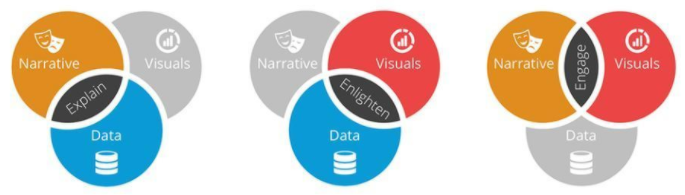
\includegraphics[width=7cm]{./imagenes/i2.png} 
\end{center}

En cada gráfico las interacciones de los elementos significan cosas diferentes, con resultados particulares. Como resultado vemos las siguientes interacciones:\\ \\
\textbf{ Narrativa y datos } 
\\La combinación de ambos sirve para ofrecer a la audiencia una explicación sobre los mismos.\\\\
\textbf{ Visualización y datos } 
\\Como ves en la imagen, la palabra enlighten (que significa iluminar) es el resultado de la combinación de ambos. Añadir una visualización a los datos ayuda informar de forma entretenida e inteligible.\\\\
\textbf{ Narrativa y visualización}
\\Esta combinación tiene como resultado la captación de clientes.\\ \\ 


Si los elementos estan combinados correctamente, el resultado será un Data 
Storytelling que conduzca al cambio positivo del negocio. Lo importante es 
que la audiencia sea capaz de entender y recordar el mensaje que se quiere 
transmitir, por eso los profesionales del Big Data y el Storytelling deben 
conocer bien a sus audiencias para saber qué ofrecer.[3]

\subsubsection{¿Por qué es importante el Data Storytelling?}
Cinco son las razones: \\
\textbf{ Contexto } 
\\Es la forma en la que se da sentido a los 
datos, proporciona perspectiva e interpretación
 de la información ya que ayuda a simplificar y 
 hacer que los datos sean más significativos, 
 relevantes e interesantes.\\\\
\textbf{ Entendimiento } 
\\Es la vía más sencilla para hacer entender a 
los demás la importancia de los datos y para ello,
 se requiere siempre de una historia.\\\\
\textbf{ Confianza } 
\\ Las historias que incorporan datos y análisis
 son siempre más convincentes que las basadas en 
 anécdotas o experiencias personales. \\\\
\textbf{ Simplicidad } 
\\Consigue una representación más abreviada del 
análisis de datos al poder simplificar la 
información los frente a los beneficiarios, 
reduciendo el tiempo de exposición, encajando 
las historias de forma breve y rápida.\\\\
\textbf{ Estandarización } 
\\Ayuda a difundir los resultados al
 establecer patrones dentro de la información 
 al expresar fácilmente actividades analíticas 
 en historias.[4]\\\\


\subsubsection{Rol del traductor de datos}

Muchas empresas comienzan a incorporar la figura del “traductor de datos” para hacer entendible los descubrimientos basados en datos. Este traductor, por medio del Storytelling, le da un sentido a los datos mientras muestra los resultados en un dashboard o en un powerpoint con gráficas.  

El traductor tiene que preguntarse cómo crear una historia interesante para que la audiencia la entienda. Es por eso que son importante las técnicas narrativas del periodismo, como las famosas 5W (quién, dónde, cuándo, cómo y por qué).

\subsubsection{Ventajas}
\begin{itemize}
	\item \textbf{Identificar y actuar rápido sobre tendencias emergentes:}incluso los archivos de datos casi infinitos empiezan a tener sentido al representarse gráficamente; lo que nos permite detectar parámetros que están altamente correlacionados.
	\item \textbf{Comprensión ágil de la información:} las representaciones gráficas permiten ver grandes cantidades de datos de forma clara y coherente, lo que facilita la extracción de conclusiones e insights.
	\item \textbf{Crear un nuevo lenguaje de negocio para contar la historia a otros:} una vez que hemos descubierto nuevos insights, el siguiente paso es comunicarlos a través de gráficos simples o visualizaciones elaboradas para lograr engagement. 
	\item \textbf{Encontrar relaciones y patrones dentro de los activos digitales:} descubrir tendencias dentro de los datos nos puede dar una ventaja competitiva, como detectar puntos clave que están afectando a la calidad del producto o solucionar problemas antes que se vuelvan más complicados.[5]
\end{itemize}
\subsubsection{Data Storytelling con Power BI}

Es una solución de análisis empresarial que permite visualizar los datos y compartir información con toda la organización. Incluso se pueden incorporar las visualizaciones en tu aplicación o sitio web; para ello Power BI nos permite conectarnos a cientos de orígenes de datos para hacerlos más entendibles con paneles e informes dinámicos, personalizados e interactivos.
Las personas entendemos mejor con historias que sólo recibiendo datos. En realidad, nos interesamos más cuando hay un contexto de por medio, que más allá de mostrar datos, nos dé información sobre algún suceso por el que sea necesario analizar y tomar decisiones.
Objetivamente, se trata de traducir los datos a un lenguaje más de negocio, de manera que sean entendibles para todos ya que generar reportes sin claridad en lo que buscamos transmitir o informar será inútil para nuestros proyectos. Todo esto nos lleva a desarrollar el Data Storytelling.
\begin{center}
	
\includegraphics[width=7cm]{./imagenes/bi.png} 
\end{center}	
Power BI como herramienta nos presenta algunas herramientas para usar en búsqueda de crear informes interactivos, personalizados y Storytelling como:
		*Bookmarks
		* Buttons
		*Page Report Tooltip
		* Drill Through\\
	

\textbf{Ejemplo}
\\Digital Phone es una empresa que se encarga de vender telefonía móvil y servicios de operadores a empresas distribuidoras, que se encuentran categorizadas en base a la venta y utilidad que les genera, en dos grandes grupos denominados Gold y Silver. Digital Phone es un intermediario entre, las operadoras y marcas de telefonía como LG, Motorola, Xiaomi, etc, y los principales distribuidores como Metro, Wong, etc. Por lo que necesita analizar las ventas generadas por cada distribuidor, operador, marca y modelo, realizando incluso una comparación con el mes anterior al del análisis.
\textbf{Bookmarks}, en la parte superior derecha, que nos permite redireccionar a otra página para analizar las ventas por distribuidor u operador dependiendo de la elección que realice en el reporte.
\begin{center}
	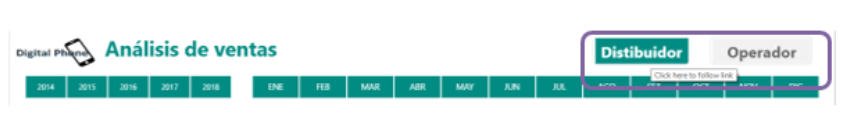
\includegraphics[width=7cm]{./imagenes/i3.png} 
\end{center}

\textbf{Buttons}, en la parte superior derecha, que me permite regresar a la página principal luego de haber navegado por los bookmarks.
\begin{center}
	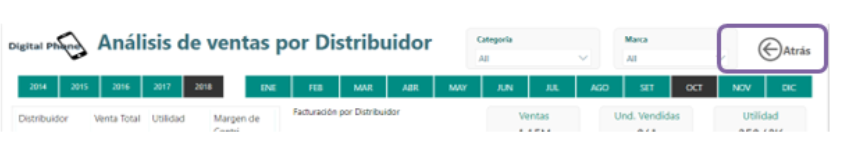
\includegraphics[width=7cm]{./imagenes/i4.png} 
\end{center}

\textbf{Page Report Tooltip},, usados en el gráfico de ventas por categoría y margen Contribución, ventas y utilidad por país, para concer un detalle más personalizado.
\begin{center}
	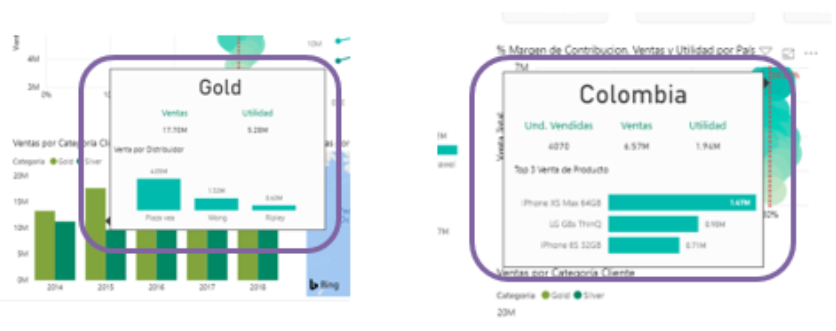
\includegraphics[width=7cm]{./imagenes/i5.png} 
\end{center}

\textbf{Drill Through}, en la tabla de operadores luego de haber navegado por el bookmarks de operador, para obtener detalles de la venta por operador más personalizados y con gráficos distintos.
\begin{center}
	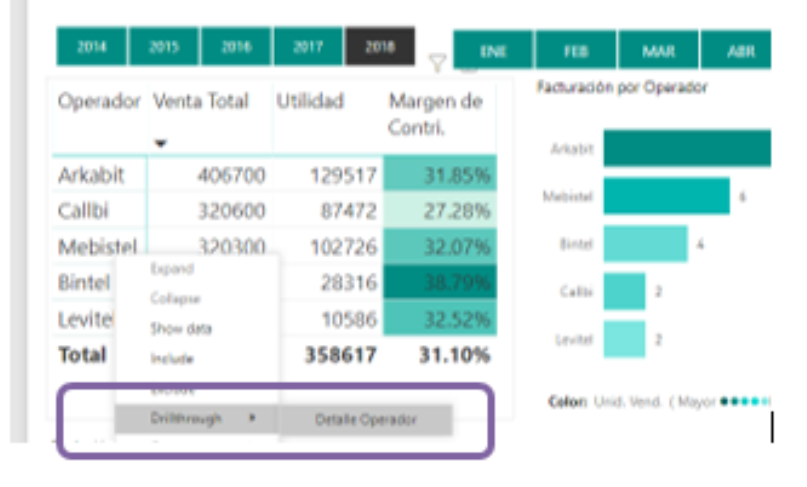
\includegraphics[width=7cm]{./imagenes/i6.png} 
\end{center}

\textbf{Herramientas de Data Storytelling}
\textbf{Data Stories Gallery:} 
\\Contiene una galería de ejemplos para navegar y
 empezar a generar nuevas ideas de reportes que se 
 podrían construir.\\\\

\textbf{Report Themes:} 
\\Son temas de colores ya definidos que pueden utilizarse 
en los reportes, para evitar buscar colores o darle colores 
a cada gráfico o reporte.\\\\

\textbf{Templates Layouts:}
 \\Son plantillas de fondo que permiten ser usados como
  base para sobre ellos empezar a ordenar y darle un 
  esquema a las visualizaciones de nuestros informes.[6]\\\\


  \subsubsection{Data Storytelling con python}
  
  La biblioteca llamada pandas es un paquete de Python que proporciona estructuras de datos y es útil para datos estructurados y de series temporales. Funciona principalmente con Series (para 1 dimensión) y DataFrames (para 2 dimensiones). El uso de pandas es bastante eficiente en el análisis inicial de nuestros datos.
  \begin{center}
	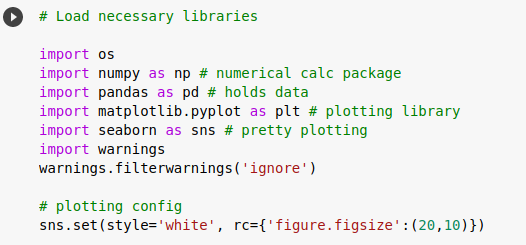
\includegraphics[width=7cm]{./imagenes/p1.png} 
\end{center}


Inicialmente podemos inspeccionar la cantidad de datos y el tipo de tipos de datos que estamos tratando con el uso de una serie de métodos bajo el objeto df.
\begin{center}
	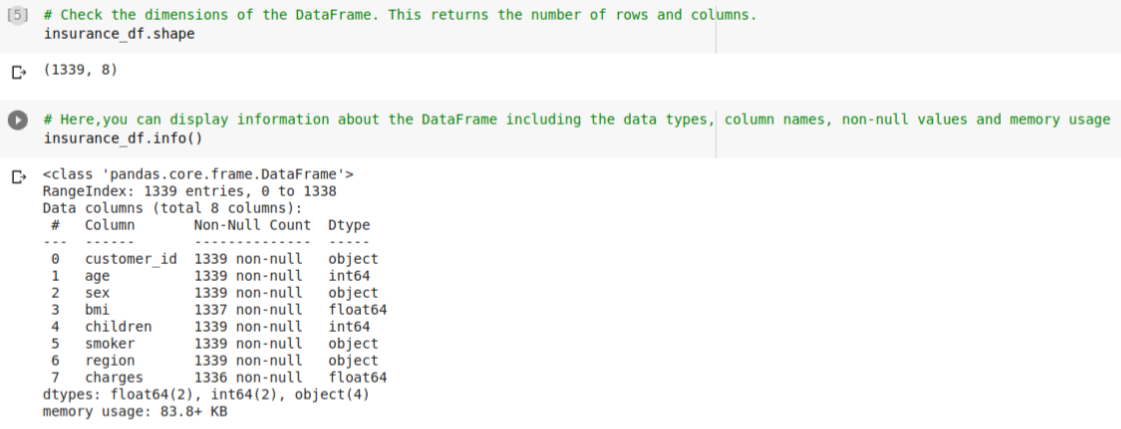
\includegraphics[width=7cm]{./imagenes/p2.png} 
\end{center}

A continuación, generamos estadísticas descriptivas para nuestros datos para que podamos comprobar los promedios, los valores extremos y la dispersión de nuestros puntos de datos. Esto se logra fácilmente mediante describe().
\begin{center}
	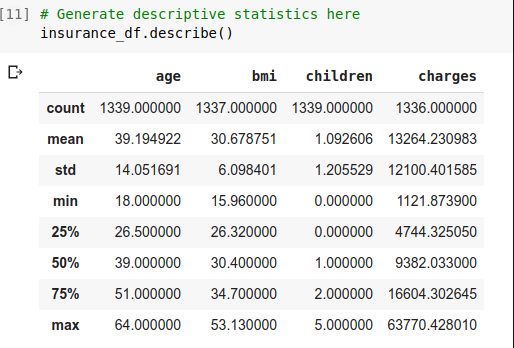
\includegraphics[width=7cm]{./imagenes/p3.png} 
\end{center}

La trama es la parte más importante de una historia. Aquí es donde llegamos a conocer y ver las relaciones entre los personajes. Aquí es donde vemos toda la acción. 
Aquí es donde Matplotlib y Seaborn entran en la imagen.
\begin{center}
	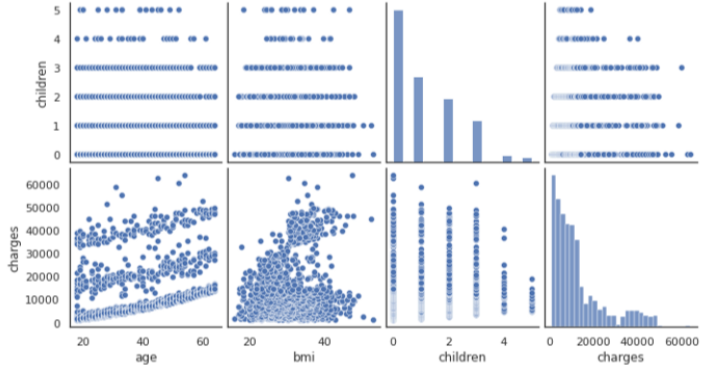
\includegraphics[width=7cm]{./imagenes/p4.png} 
\end{center}

Se puede utilizar para predecir la prima para un cliente en función de varios factores. Basándonos en las tramas, podemos decir que los cargos por edad y seguro tienen una correlación positiva que podemos explorar aún más. Este es un buen punto de partida.
Los histogramas pueden darnos una visión rápida de cómo se distribuyen nuestros puntos de datos.Como se ve en la imagen de abajo.
\begin{center}
	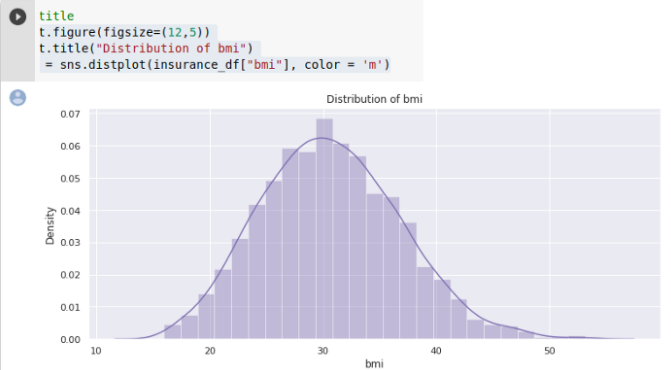
\includegraphics[width=7cm]{./imagenes/p5.png} 
\end{center}
Las propiedades de estos gráficos y la exposición a estas bibliotecas pueden ayudar a alguien a conseguir la caída de la creación de visualizaciones impresionantes en Python.

  \section{CONCLUSIONES}
  Data Storytelling consiste 
  en un enfoque estructurado sobre cómo comunicamos
   insights a partir de los datos. Para las organizaciones
	es muy importante incluir historias en los análisis, 
	debido a que ayuda a un fácil entendimiento y a persuadir 
	para generar un cambio en las acciones de las personas. 
	El rol de traductor de datos permite hacer entendible los 
	descubrimientos basados en datos, así como también aplicar
	 distintas estrategias periodísticas. Desarrollar habilidades en comunicación, en escucha y oratoria es importante para que
	  Data Storytelling tenga un éxito asegurado.[6]

\section{RECOMENDACIONES}

\textbf{Empieza por el final}
\\Las historias tienen comienzo, desarrollo y un final que cierra la historia y que es, muchas veces, la razón por la que los receptores se han mantenido atentos al mensaje. Pero en el mundo de los negocios y de los mensajes de empresa no hay que seguir necesariamente ese criterio. De hecho, ni siquiera en los mensajes 'artísticos', como puede ser la literatura, se hace. A veces empezar por el final y luego remontarse a la historia puede funcionar muy bien, porque ayuda a que la audiencia se centre en lo que le estás contando y no tanto en intentar averiguar hacia dónde esta historia los llevará.
\\\\
\textbf{Es importante que la historia sea memorable, pero también que sirva para los objetivos de la empresa}
\\
Una de las cuestiones que siempre se repiten cuando se habla de marketing de contenidos y de storytelling es que lo que se está contando tiene que ser memorable. La narración tiene que conseguir colarse en la memoria de los consumidores y asentarse entre sus recuerdos, lo que hace que se centre muchas veces el grueso de los recursos en este punto.

Pero lo cierto es que no solo es importante crear una buena historia y una historia que se recuerde, sino que además esta tiene que estar en línea con lo que la empresa quiere de ella. ¿Cuál es el objetivo de la historia? ¿Qué espera la marca con su esfuerzo en storytelling? El objetivo se convierte así en crucial y en decisivo para el éxito o no del esfuerzo.
\\\\
\textbf{Ponte en los zapatos de tu consumidor}
\\O, lo que es lo mismo, analiza la historia desde la perspectiva de tu audiencia. Es crucial que la historia se adapte a lo que la audiencia a la que va destinada quiere y necesita y por tanto un buen storytelling siempre tiene en cuenta a quién está al otro lado.
\\\\
\textbf{Resume tu historia}
\\Esto no implica que la historia tenga que contarse en un par de palabras, sino más bien que cuando se esté construyendo se sea capaz de hacerlo. Un buen novelista o un buen guionista es capaz de decir de qué va su libro o su película en pocas frases. Como apuntan en el análisis, si no se es capaz de resumir lo que se está queriendo contar en un tuit, algo se está haciendo mal en el storytelling.
\\\\
\textbf{Encuentra al malo de tu historia}
\\Hay que encontrar el problema que hará que la historia avance y que la audiencia conecte con ella. No hay más que pensar en las películas de éxito: el protagonista siempre tiene un antagonista (que no necesariamente tiene que ser un villano).
\\\\
\textbf{No olvides la regla básica de contar historias}
\\El principio, desarollo y final funcionan porque ayudan a crear un storytelling limpio y uno que permite organizar bien lo que se está narrando y seguirlo fácilmente por parte de la audiencia.
\\\\

\begin{thebibliography}{} 

	\bibitem[Introducción al Storytelling, 2019]{} 
	\newblock  Recuperado de :url{https://www.compartirpalabramaestra.org/actualidad/articulos-informativos/introduccion-al-storytelling} [1]

	\bibitem[Socialmood (2020]{} 
	\newblock  ¿Qué es el storytelling?-Diccionario de Marketing. 40deFiebre. url{https://www.40defiebre.com/que-es/storytelling}[2]
	
	\bibitem[Galiana, P. (2020, 8 enero)]{} 
	\newblock  Data Storytelling, qué es y cómo puede mejorar tu estrategia de contenidos. Thinking for Innovation. url{https://www.iebschool.com/blog/data-storytelling-que-es-big-data/}[3]

	\bibitem[A. (2020, 17 abril)]{} 
	\newblock  Por qué es tan necesario el Data Storytelling. Prometeus Global Solutions. url{https://n9.cl/vytvs}[4]

	\bibitem[Crespo, P. R. (2020, 7 septiembre)]{} 
	\newblock Lo que necesitás saber sobre Data Storytelling. Data IQ. url{https://dataiq.com.ar/blog/lo-que-necesitas-saber-sobre-data-storytelling/} [5]
	
	\bibitem[Data Storytelling con Power BI. (2021, 4 enero)]{} 
	\newblock Kaits Consulting. url{https://www.kaitsconsulting.com/storytelling-power/}[6]

	\bibitem[Derilo, R. (2020, 23 octubre)]{} 
	\newblock  Derilo, R. (2020, 23 octubre). Adventures with Python: Storytelling with pandas and Matplotlib (ft. Seaborn). Medium.url{ https://medium.com/analytics-vidhya/adventures-with-python-storytelling-with-pandas-and-matplotlib-ft-seaborn-64161e3f1431}[7]
	
\end{thebibliography}




\end{document}
